

\documentclass[11pt,twoside,a4paper]{cernrep}
\usepackage{fcc_common}
\usepackage{amssymb}
\usepackage[final]{epsfig}
\usepackage{color}
\usepackage{xcolor}
\usepackage{graphicx}
\usepackage{lineno}
\usepackage{verbatim}
%\usepackage{natbib}
%\newcommand{\textmu}{$\mu$}
%\newcommand{\textnu}{$\nu$}
%\newcommand{\texttau}{$\tau$}
%\newcommand{\textgamma}{$\gamma$}
\newcommand{\hl}{}
%\newcommand{\textpi}{$\pi$}
\newcommand*{\effg}{\ensuremath{\epsilon_{\gamma}}}
\newcommand*{\misg}{\ensuremath{\epsilon_{j \rightarrow \gamma}}}
\newcommand*{\effb}{\ensuremath{\epsilon_{b}}}
\newcommand*{\misl}{\ensuremath{\epsilon_{l \rightarrow b}}}
\newcommand*{\misc}{\ensuremath{\epsilon_{c \rightarrow b}}}
\newcommand*{\mislc}{\ensuremath{\epsilon_{l(c) \rightarrow b}}}
\newcommand*{\maa}{\ensuremath{m_{\gamma\gamma}}}
\newcommand*{\mbb}{\ensuremath{m_{bb}}}

\newcommand{\MS}[1]{\textbf{\textcolor{purple}{MS - #1}}}
\newcommand{\MLM}[1]{\textbf{\textcolor{blue}{MLM - #1}}}
\newcommand{\CH}[1]{\textbf{\textcolor{green}{CH - #1}}}



\begin{document}
%%%%%%%%%%%%%%%%%%%%%%%%%%%%%%%%%%%%%%%%%%%%%%%%%%%%%%%%%%%%%%%%%
%%%%%%%%%%%%%%%%%%%%%%%%%%%%%%%%%%%%%%%%%%%%%%%%%%%%%%%%%%%%%%%%%

\MS{still missing all the references to the various CDS notes and detector cosmetics.}

\section{Detector Performance and Physics Benchmark Studies}

Physics at the FCC-hh will involve final states with momenta ranging from a few tens of GeV to tens of TeV. The high end of the spectrum features searches for resonances at the highest possible mass (up to 40 TeV) decaying into multi-TeV leptons ($\ell=$~e, \textmu), tau's, light/heavy quarks and gauge bosons. High momentum decay products such as muons, electrons, photons, or charged hadrons can be used to define minimal requirements on tracking and calorimetry energy/momentum resolution. Multi-TeV unstable heavy objects such as gauge bosons, top or bottom quarks and tau leptons that decay into highly boosted and collimated stable particles are instead useful benchmarks for constraining the angular separation power of the detector, in particular of the tracker and the calorimeters. At such high $p_{T}$ the relative impact of pile-up can be neglected as a first approximation.
The detector performance at low $p_{T}$ is instead fixed by targeting maximal precision on measurements at threshold and by requiring the best sensitivity to searches involving compressed or low mass spectra. The goal is to define a targets for object reconstruction efficiencies and fake-rate as well as energy-momentum resolution at low momentum, in a regime where the relative impact of the pile-up is large.

A complete discussion of the physics opportunities at the FCC-hh can be found in Volume 1. In this section we focus on a small selection of physics studies that played a key role in defining the target performance for the FCC-hh baseline detector presented in the previous sections and in shaping the detector design. The measurement of the Higgs self-coupling is presented, together with a discussion on the impact of pile-up on the measurement. A Z$^{\prime}$ into di-lepton search and a fully hadronic stop search are then discussed. These searches define the momentum and angular resolution for multi-TeV leptons and boosted hadronic jets. Finally, a search for \emph{disappearing tracks} is presented, with a focus on the inner tracking detector design.

In the studies presented here, Monte Carlo samples have been generated with the {\scshape MG5\_}a{\scshape MC@NLO}~2.5.2 package, showered and hadronised with {\scshape Pythia}~8.230. With the exception of the disappearing track study, the detector simulation was performed with the fast simulation framework {\scshape Delphes}~3.4.2 where the sub-detector specifications defined in the previous sections have been parameterised. Rather than simulating the pile-up directly in fast simulation, we have studied its possible impact on the final sensitivities through its indirect effects on specific object performances. The disappearing track study uses instead custom simulation  pile-up simulation and track clustering algorithm.

\subsection{The Higgs Self-coupling}

A precise measurement of the Higgs self-coupling $\lambda$ is crucial for constraining the shape of the Higgs potential near our vacuum. The self-coupling can be determined from non-resonant di-Higgs production. It is an extremely challenging measurement because of the small di-Higgs production cross-section (at $\sqrt{s} {=}100$ TeV, $\sigma_{gg\to {\rm HH}} \approx 1.5$ pb). The $\rm b\bar{b}$\textgamma\textgamma~ decay mode is the most promising channel despite the small branching ratio of 0.25\%. The main backgrounds for this measurement are single Higgs production, \textgamma\textgamma+jets, and \textgamma+jets.

The photon identification efficiency is assumed to be $\effg=$~95\% for $|\eta| < 2.5$ and $\effg=$~90\% for $2.5 < |\eta| < 4.0$. The light jet to photon mis-identification probability (fake-rate) is parameterised by the function $\misg = 0.002 \exp(-p_T[\mathrm{GeV}]/30)$. The b-tagging efficiency $\effb$ and the light (charm) mistag rates $\mislc$ are assumed to be $\effb=$~85\% and $\mislc=$~1 (5)\%.

The events are selected if they contain two isolated photons and two b-tagged jets. Additional selection criteria are applied to suppress backgrounds, such as requiring for the di-photon and di-jet pairs $p_T$(\textgamma\textgamma,bb) > 100 GeV. The invariant mass of the $\rm b\bar{b}$ pair is required to be within \linebreak \mbox{$100 <m_{\rm bb} < 130$ GeV}.

The signal is extracted via a 2D fit on the photon pair and the Higgs pair invariant masses, $m_{\mbox{\textgamma\textgamma}}$ and $m_{\mbox{\textgamma\textgamma}\rm b b}$ using analytical parametrisations for the signal and background shapes. Figure~\ref{higgs}(a) shows that with a $1\%$ systematic uncertainty on the signal cross-section and the single Higgs background normalisation, $\lambda$ can be measured with a precision of 6.5\% (at 68\% confidence level) with an integrated luminosity of 30 ab$^{-1}$. The single most important variable that controls the sensitivity of this measurement is the di-photon pair invariant mass.
In accordance with Figure 7.17 b) \MS{fix by linking to actual figure} , the di-photon invariant mass resolution is found to be $\delta m_{\gamma\gamma}\approx 1.3$~GeV with 0 PU and $\delta m_{\gamma\gamma}\approx 2.9$~GeV with 1000 PU. The resulting impact on the Higgs self-coupling precision, shown in Figure~\ref{higgs}b, is found to be of order 1\%. The assessment of the impact of pile-up on the photon energy resolution has to be considered as conservative. Indeed, the use of timing information as well as the optimisation of the photon clustering using deep learning techniques is expected to bring large improvements in terms of pile-up rejection. We also point out that the precision of the Higgs self-coulpling measurement will be benefit from the combination with other Higgs decay modes such as bb\texttau\texttau, and bb4$\ell$.
%
\begin{figure}
  \centering
  a)
  %\includegraphics[width=0.42\columnwidth]{\main/experiments/img/hh_syst.pdf}
  \includegraphics[width=0.42\columnwidth]{hh_syst.pdf}
  b)
  %\includegraphics[width=0.42\columnwidth]{\main/experiments/img/hh_gamma.pdf}
  \includegraphics[width=0.42\columnwidth]{hh_gamma.pdf}
  \caption{ a) Expected precision on the Higgs self-coupling modifier $\kappa_{\lambda}{=}\lambda_{obs}/\lambda_{SM}$ with no systematic uncertainties (blue), $1\%$ signal uncertainty (red) and with $1\%$ uncertainty on the ttH background (green). b) Comparison of the precision on $\kappa_{\lambda}{=}\lambda_{obs}/\lambda_{SM}$ obtained by assuming either nominal $\delta m_{\mbox{\textgamma\textgamma}} {=}1.3$~GeV (0PU) or degraded $\delta m_{\mbox{\textgamma\textgamma}}{=}2.9$~GeV (1000 PU) di-photon invariant mass resolution.}
  \label{higgs}
\end{figure}

\subsubsection{High Mass resonances decaying to leptons}

New Physics models with extended gauge groups often feature additional U(1) symmetries with corresponding heavy spin-1 bosons. These bosons, generally referred to as Z$^{\prime}$, manifest as a very narrow resonance \mbox{($\Gamma/m \sim 1-2\%$)} through their decay to two high energy SM particles. These searches typically involve reconstucting an invariant mass peak as a proxy for the Z$^{\prime}$ resonance. An excellent energy momentum resolution is needed in order to achieve the highest possible discovery reach.

The decay products of heavy resonances are in the multi-TeV regime and the capability to reconstruct their momentum imposes stringent requirement on the detector design. For simplicity, we consider here only the Z$^{\prime}\rightarrow \ell\ell$ decays, where $\ell=$~e, \textmu.
Reconstructing the track curvature of multi-TeV muons requires excellent position resolution and a large lever arm. In Figure 7.21  - \MS{fix by linking to actual figure} it is shown that the current tracking plus muon design allows for an outstanding $p_T$ resolution $\sigma(p_T)/p_T~\approx~10\%$ for $p_T=20$~TeV. Reconstructing multi-TeV electrons requires an EM calorimeter design with a small constant term, which is ensured with a highly uniform calorimeter with no leakeage. The present EM design ensures an excellent $\sigma(E)/E~\approx~0.2\%$ at multi-TeV energies, as shown in Figure 7.17 a) - \MS{fix by linking to actual figure}.

The Z$^{\prime}$ boson in the Sequential Standard Model (SSM), with couplings identical to those of the SM Z boson is taken as a benchmark. Events are selected by requiring two high $p_{T}$ isolated leptons with $p_T(\ell)>6$ TeV with $|\eta(\ell)|<3$. The only significant background is the di-lepton continuum background. A 50\% systematic uncertainty on the background rate is assumed. The signal extraction is performed via a profile likelihood fit on the di-lepton invariant mass. The di-muon spectrum for a $m_{\rm Z^{\prime}} {=} 40$~TeV is illustrated in Figure~\ref{zprime}a). The discovery reach for the separate and combined di-lepton channels is shown in Figure~\ref{zprime}b.
the discovery reach in the di-electron and di-muon channel is comparable. Despite the worse resolution at high momenta, the reach in the di-muon channel is similar to that in the di-electron channel, because of the rapidly falling background yields at very large invariant masses. We can thus conclude that the present muon performance is close to optimal and saturates the physics potential of the FCC-hh at high $p_T$ . With the current detector design, the combination of the e$^+$e$^-$ and \textmu$^+$\textmu$^-$ channels allows for a Z$^{\prime}$ discovery with a mass up to $m_{\rm Z^{\prime}} {=} 42$ TeV.

%
%
%
\begin{figure}
  \centering
  a)
  %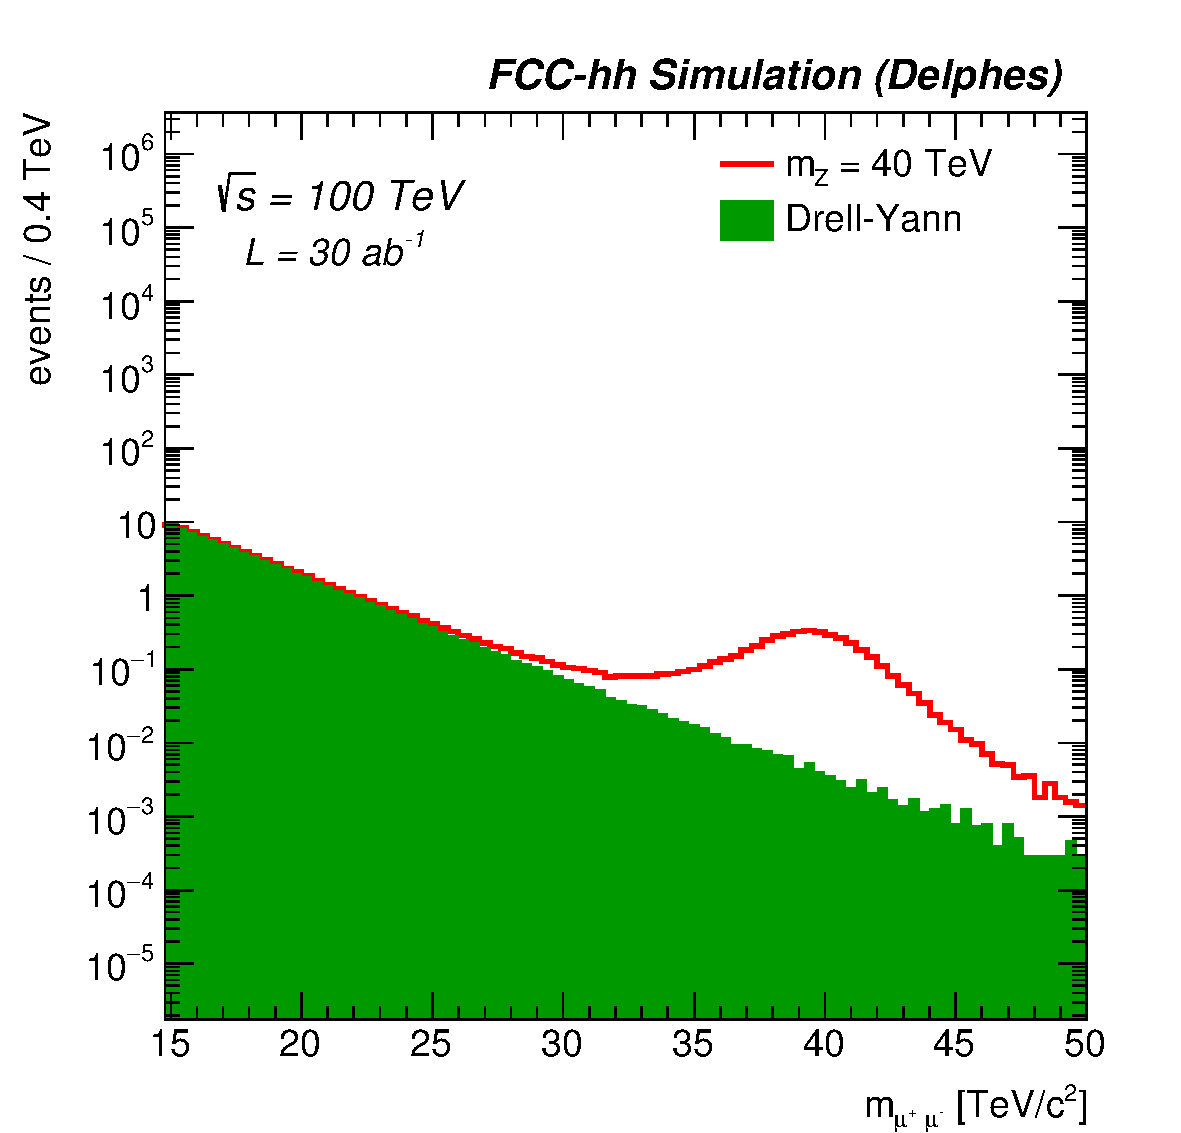
\includegraphics[width=6cm]{\main/experiments/img/mmumu.eps}
  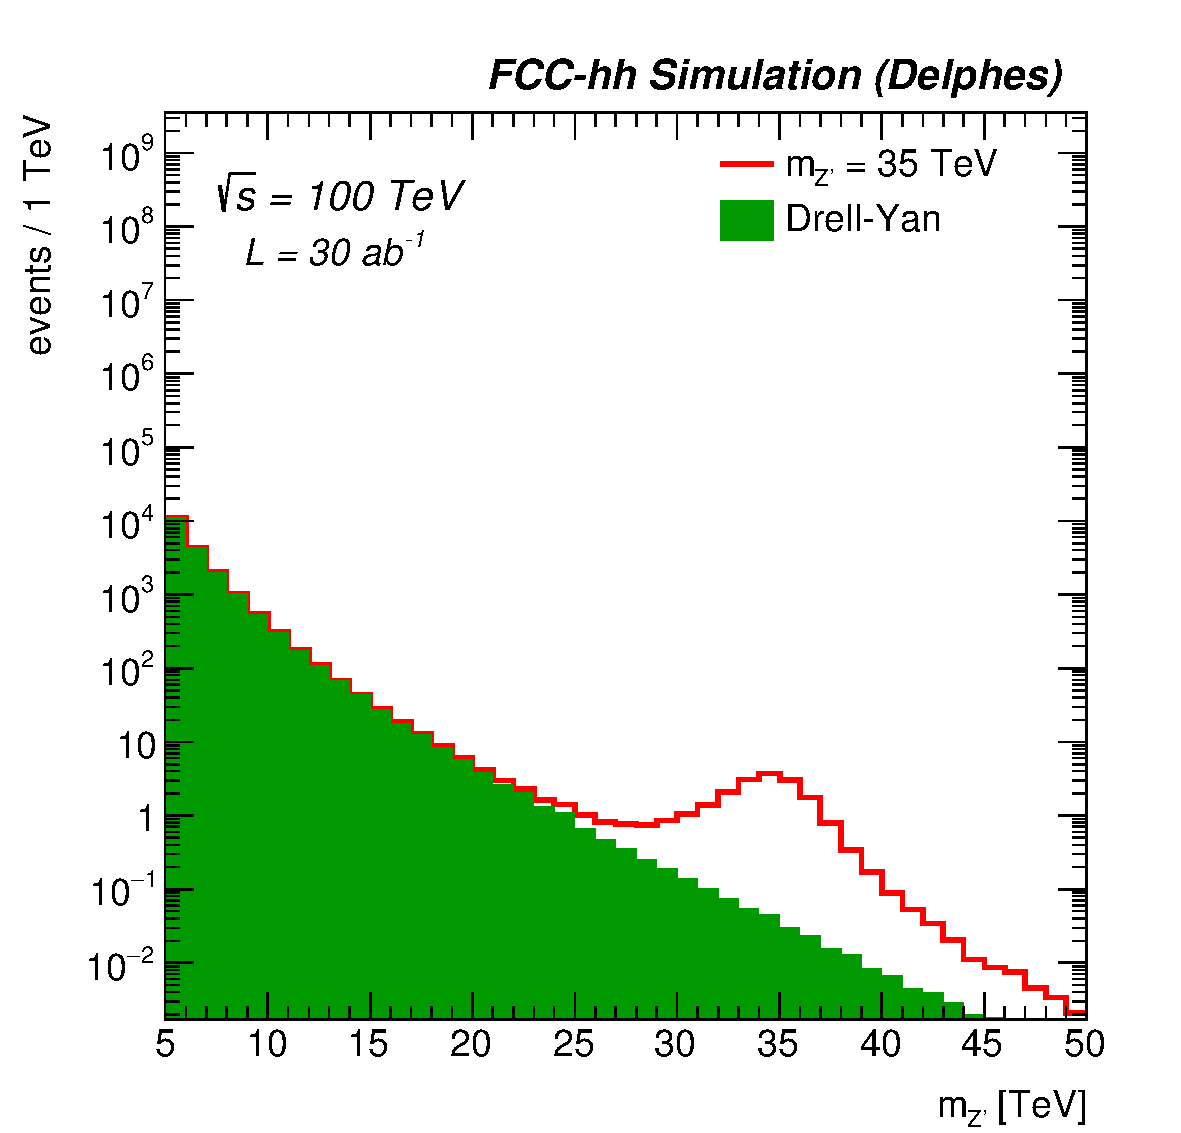
\includegraphics[width=6cm]{mzp_sel0_stack_log.eps}
  b)
  %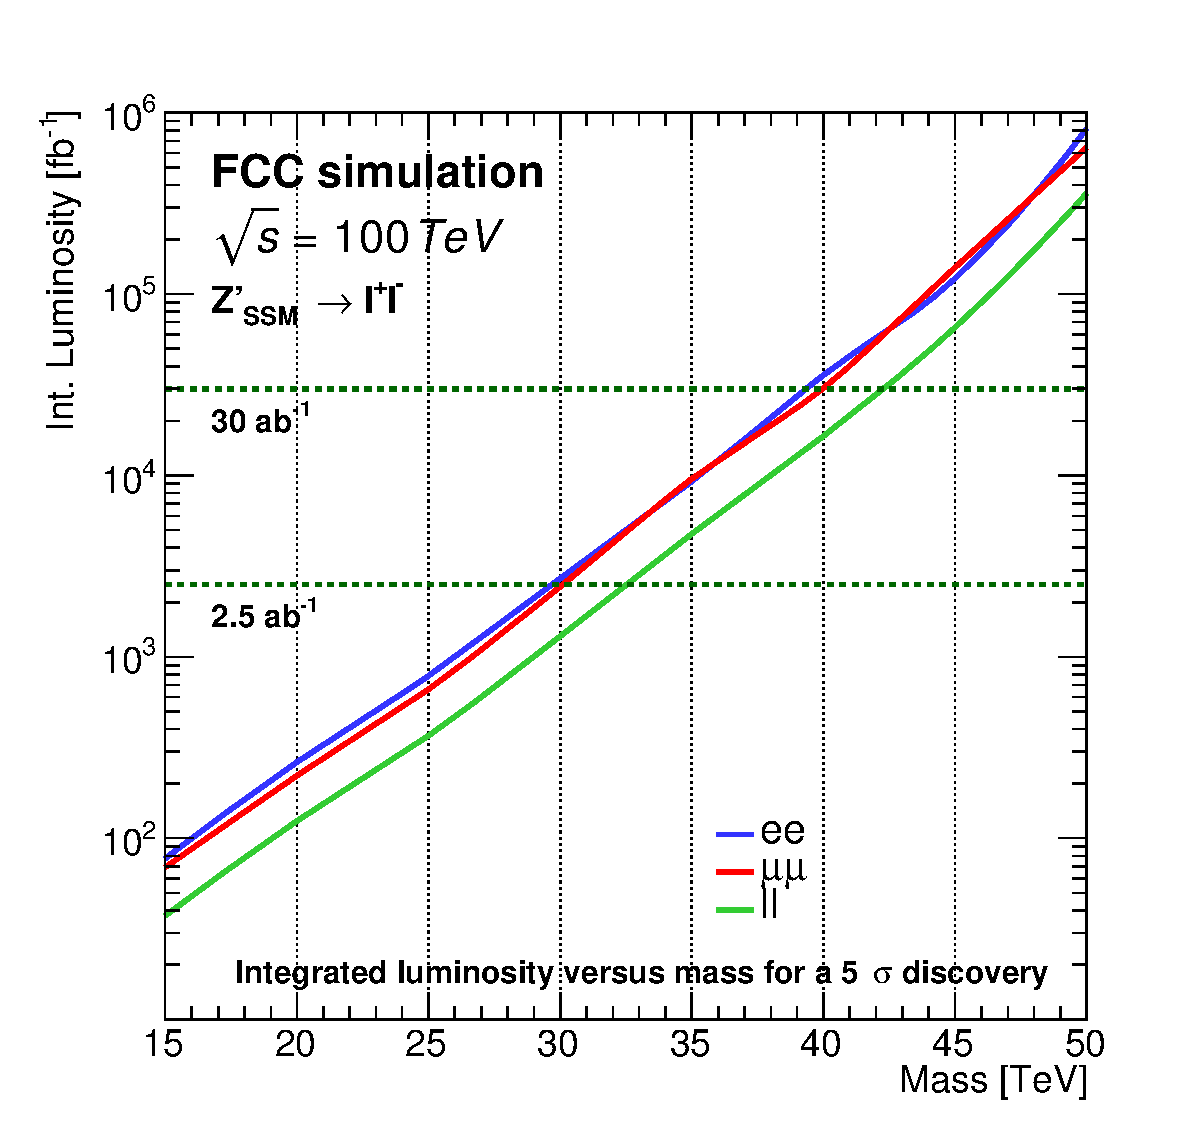
\includegraphics[width=6cm]{\main/experiments/img/disc-zp.eps}
  \includegraphics[width=6cm]{DiscoveryPotential_ll_comb_rootStyle.eps}
  \caption{a) The di-muon invariant mass spectrum for a signal of $m_{\rm Z^{\prime}} {=} 40$~TeV and background. The background is displayed with a solid histogram and the distribution of the signal model is shown with solid red line. The expected yields are scaled to 30\,ab$^{-1}$. b) Integrated luminosity as a function of the 5$\sigma$ discovery reach for the e$^+$e$^-$, \textmu$^+$\textmu$^-$ channels and their combination.}
  \label{zprime}
\end{figure}


\subsection{Top Squarks}

Supersymmetry is a theoretical framework that can address the hierarchy problem, allows for the unification of couplings at high energies and provides a natural dark matter candidate, often the lightest neutralino. The production of top squarks (stop) is studied through pp$\rightarrow \tilde{\rm t} \tilde{\rm t}$, in the R-parity conserving $\rm \tilde{t} \rightarrow t + \tilde{\chi}_1^{0}$ decay mode, where $\rm \tilde{t}_{1}$ is the lightest mass eigenstate of the top squark and $\tilde{\chi}_1^{0}$ is the lightest neutralino. The focus is on final states consisting of only hadronic jets. This decay mode has a striking signature: the presence of two on-shell top (t) quarks, decaying to multiple jets and b jets, and large missing transverse momentum $p_T^{\mathrm{miss}}$. At the FCC-hh, the production rate of stop pairs is sizable up to $m_{\tilde{t}} \approx 10$~TeV. For such extreme kinematics, this search is very challenging, since highly boosted top quarks will be produced in the decay of massive stop quarks, and produce jets that exhibit three extremely collimated prongs. Resolving the sub-structure inside such "top" jets is key to reject the background from QCD jets and requires excellent granularities in the tracking detectors and the calorimeters. For example, the decay products of a 5\,TeV t quark are separated by $\Delta R {=} \Delta \eta \times \Delta \phi \sim 0.05$. This number has to be compared to the angular resolution estimated at the first tracker pixel layer is given roughly by $\sigma_{\eta \times \phi} \approx 0.005$. The ECAL (HCAL) design shown in Table 7.3  - \MS{fix by linking to actual figure} ensures a granularity in $\sigma_{\eta \times \phi} \approx 0.01 (0.025)$ in the barrel. As a result, the present detector design should provide the needed angular separation power to resolve such boosted signatures.

Events are selected by vetoing electrons or muons and requiring high missing transverse energy ($p_T^{\mathrm{miss}}>2$ TeV). In addition, at least two high-$p_T$ jets ($p_T > 1$ TeV) are required, of which at least one is b-tagged ($N_{\rm b} \geq 1$), and at least one top-tagged jet ($N_{\rm t} \geq 1$). A top-tagging multi-variate discriminant for QCD background discrimination based on jet substructure observables has been developped specifically for this search by using a combination of track and calorimeter-based jet variables. It provides a working point with $\sim5\%$ mistag rate from QCD and a $\sim60\%$ top identification efficiency. The dominant SM backgrounds with intrinsic $p_T^{\mathrm{miss}}$ arise from $\rm t \bar{t}$ and $\rm t \bar{t}$V (V {=} W,Z,H) production. These backgrounds are reduced by selecting events with $|\Delta \phi({\rm t},p_T^{\mathrm{miss}})| > 0.5$.  Their contributions are estimated in dedicated control regions extrapolated to the search regions with simulation. Contributions arising from electroweak (e.g. V+jets), single t quark, ${\rm t \bar{t}} VV$ and $\rm t \bar{t} t \bar{t}$ processes represent much smaller backgrounds and will be estimated directly from simulation.

Events are divided into categories based on $N_{\rm t}$ and $N_{\rm b}$ and the shape of $p_T^{\mathrm{miss}}$ is used as the discriminating variable. Figure~\ref{stops}a shows the expected signal and background contributions in the $N_t \geq 2$ and $N_{\rm b}{=}1$ category. A simultaneous fit to signal and control regions is used to determine the exclusion potential. Figure~\ref{stops}b shows that with 30\,ab$^{-1}$ of integrated luminosity, top squarks with mass up to $\sim$10~TeV can be excluded for small that contain a not-too-heavy neutralino, regardless of the systematics scenario assumed. In comparison, at HE-LHC top squarks up $\sim$4~TeV can be exluded.
%
%
%
\begin{figure}
  \centering
  a)
  %\includegraphics[width=6cm]{\main/experiments/img/sr_1.pdf}
  \includegraphics[width=6cm]{sr_1.pdf}
  b)
  %\includegraphics[width=6cm]{\main/experiments/img/lim_30ab_comb.pdf}
  \includegraphics[width=6cm]{lim_30ab_comb.pdf}
  \caption{a) The $p_T^{\mathrm{miss}}$ distribution in background and signal events with $N_{\rm t} \geq 2$ and $N_{\rm b}{=}1$. The background processes are displayed with solid histograms and the distribution of one signal model is shown with solid red line. "LL" stands for "Lost Lepton" and collects all backgrounds where a lepton was not reconstructed due to inefficiency or limited detector acceptance. The expected yields are scaled to 30\,ab$^{-1}$. b) Exclusion potential for 30\,ab$^{-1}$ of integrated luminosity. The area to the left of and below the solid red (black) curve represents the expected exclusion and the $\pm1$ standard deviation contours for the nominal (conservative) scenario of associated systematic uncertainties. \MS{missing plot from Loukas with extrapolation to HELHC.} }
  \label{stops}
\end{figure}

\subsubsection{Disappearing Tracks}
The simple and most minimal way to include a Dark Matter candidate in the Standard Model consist in adding an SU(2) multiplet that contains a neutral state. In super-symmetry the doublet is the Higgsino and the triplet is the Wino. If DM is the neutral wino~(higgsino) and was produced in thermal equilibrium, the upper limit of the dark matter mass is determined by the observed relic abundance of dark matter: 3~TeV for the wino LSP scenario and 1~TeV for the higgsino LSP scenario. The FCC-hh provides therefore a unique opportunity to probe wino and higgsino DM.

When a pure wino/higgsino is the LSP, the mass of the \ensuremath{\tilde{\chi}_{1}^{0}}~is highly degenerate with the lightest chargino~(\ensuremath{\tilde{\chi}_{1}^{\pm}}).
Therefore, the \ensuremath{\tilde{\chi}_{1}^{\pm}}~is a long-lived state with a lifetime $\tau_{\chi}\approx 0.2~(0.023)$~ns for 3~TeV wino~(1~TeV higgsino).
A \ensuremath{\tilde{\chi}_{1}^{\pm}}~decays into a \ensuremath{\tilde{\chi}_{1}^{0}} and soft charged pion. The neutralino does not interact with the detector and the pion is too soft to be reconstructed. Therefore, the long-lived chargino can be detected as a short-distance \emph{disappearing track} with a typical length scale of $\cal{O}$(1-10)\,cm.


The backgrounds for this search can be categorised into two components.
\emph{Physical} backgrounds arise from a charged particles (electrons or charged pions) scattered by the material in the inner tracker. These are mainly W($\rightarrow \ell\nu$)+jets events, with large $E_T^{\mathrm{miss}}$~and a high $p_{T}$ track from a decay product of a W boson. The normalisation of the physical background is estimated by scaling the background rate estimated at ATLAS by the ratio of the amount of the material in the FCC tracker to that in the ATLAS inner tracker. The \emph{unphysical} background consists of fake tracks; they arise from a random combination of hits that form a short track. The fake-track rate is evaluated from simulated minimum bias events by counting the number of fake tracks passing the quality requirements. The final estimate is obtained by scaling by a pile up dependent fake rate probability. A good coverage of the volume within r~$<$~10~cm is crucial for an optimal fake-track rejection and thus for the success of this measurement.

Candidate events are required to contain at least one high $p_{T}$ jet, large \ensuremath{p_{T}^{\rm{miss}}} and no lepton~(electron or muon) with $p_{T}$ above 10~GeV.
The jet $p_{T}$ and \ensuremath{p_{T}^{\rm{miss}}}~thresholds are determined by maximising the sensitivity at each \ensuremath{\tilde{\chi}_{1}^{\pm}}~mass point based on the signal acceptance and background rate. Additionally, at least one short track~(\ensuremath{N_{\mathrm{layer}}^{\mathrm{hit}}}~$\geq$ 5) is required.

The expected significance obtained with the default tracker layout (described in Section 7.5.1 \MS{fix by linking to actual figure}) is shown in Figure~\ref{figure:SignificanceEta1} as the grey band.  The area represents an estimate of the uncertainty obtained from different QCD models of pile-up simulation. The impact of a layout with 5 pixels tracking layers instead of 4 is shown in red. Two pile-up conditions, $\left< \mu \right>$ {=} 200 and 500, have been considered to evaluate the fake-tracks background. A significance well above 5$\sigma$ for the 3~TeV wino can be reached. However, a 5$\sigma$ significance for the 1~TeV higgsino can be reached only using the alternative layout with 5 pixel layers. The sensitivity could be further improved by using the hit-timing information to suppress fake tracks or using dE/dx information to identify the velocity of the disappearing track.

\begin{figure}
  \centering
  a)
  %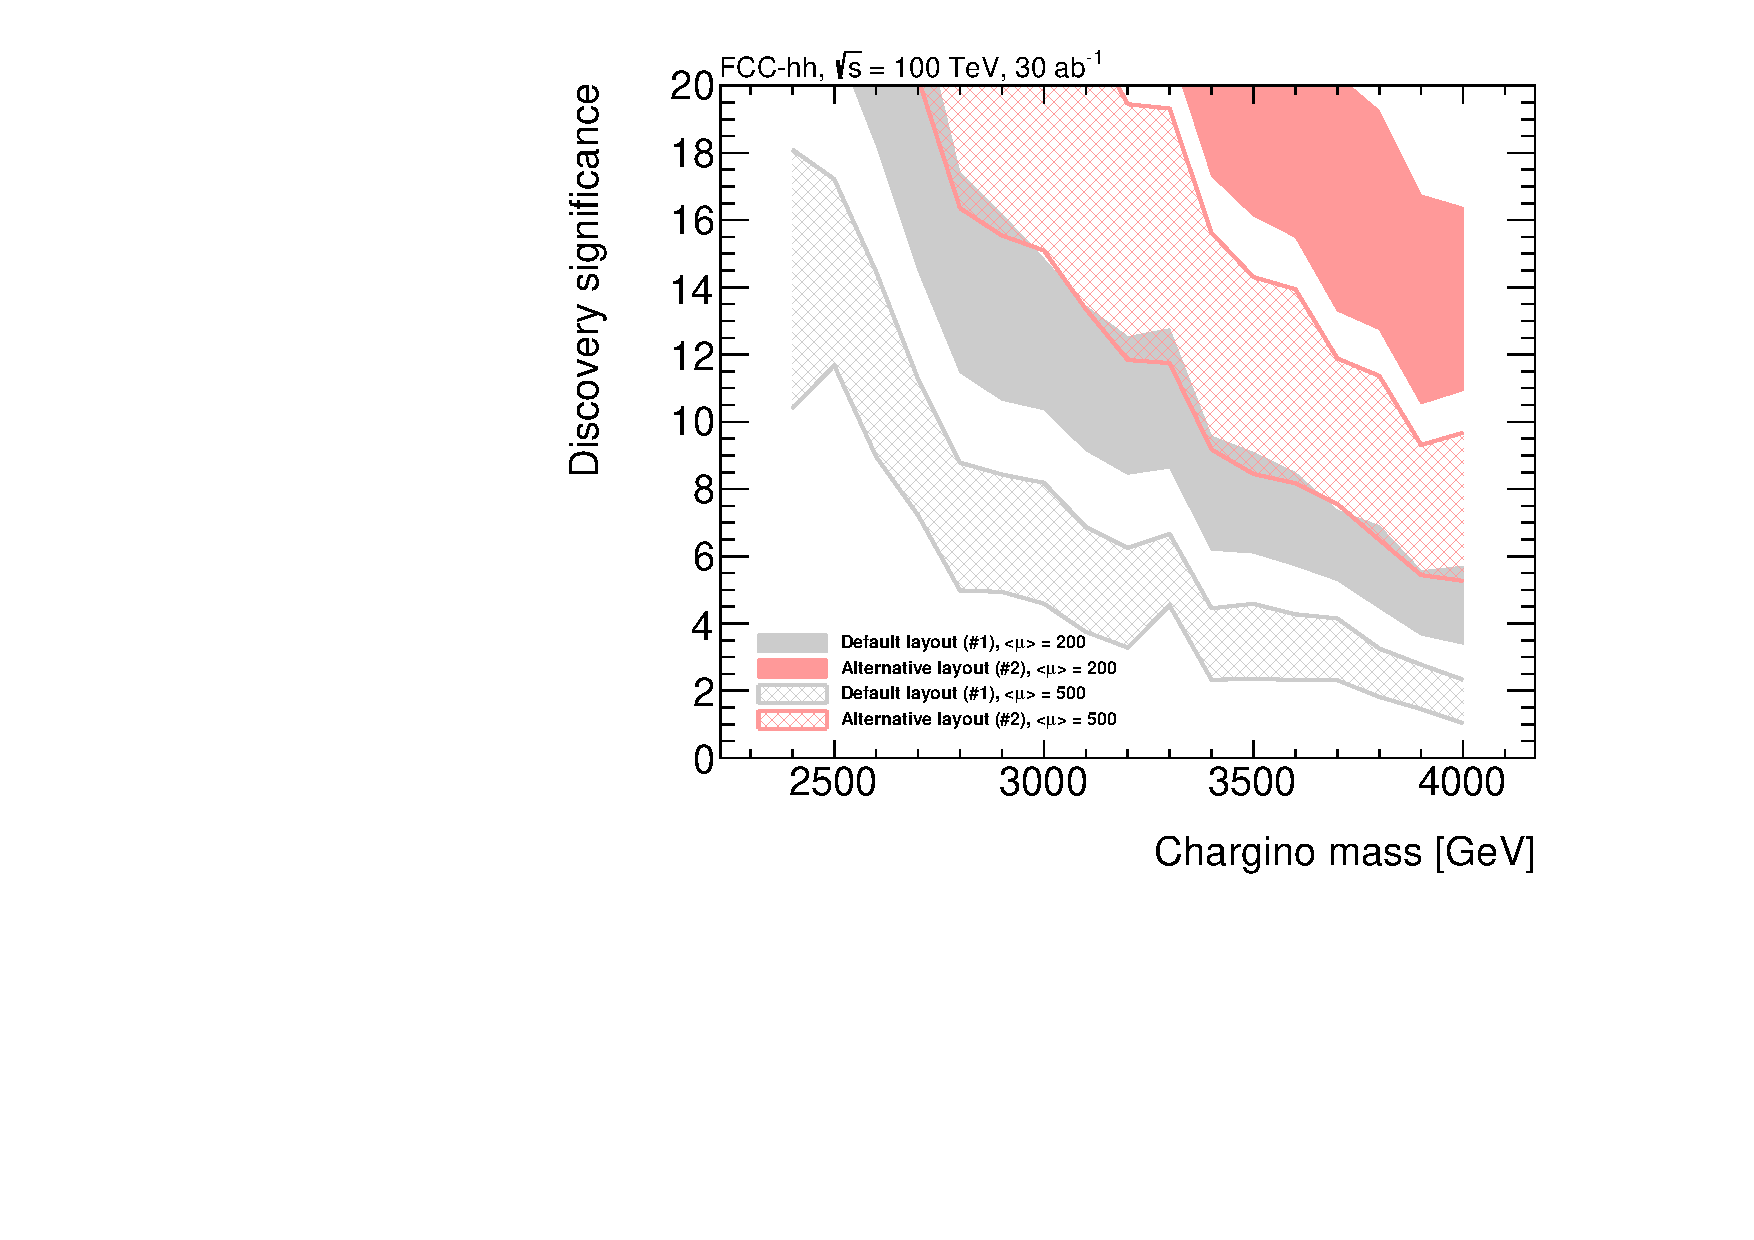
\includegraphics[width=7cm]{\main/experiments/img/h_Significance_di_wino9_eta.pdf}
  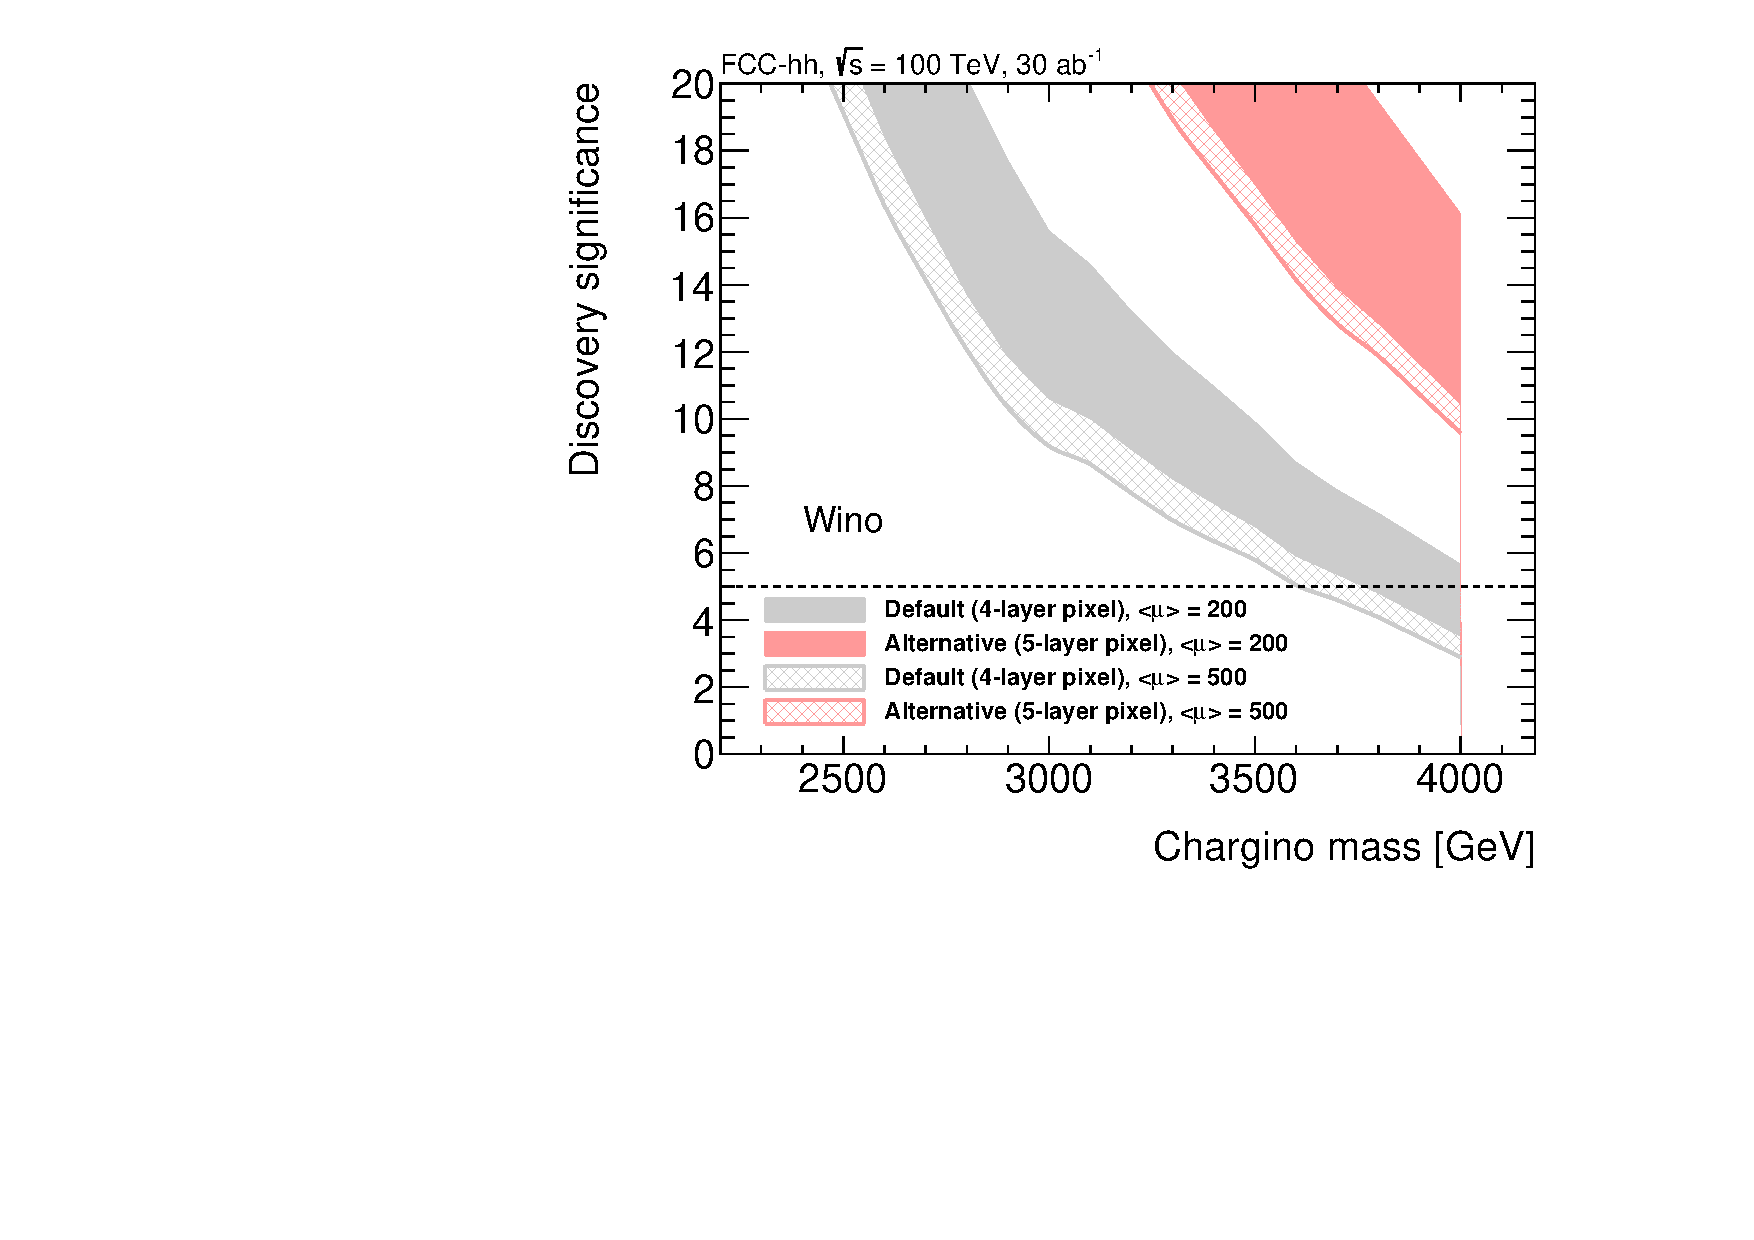
\includegraphics[width=7cm]{h_Significance_wino12_eta_5hits.pdf}
  b)
  %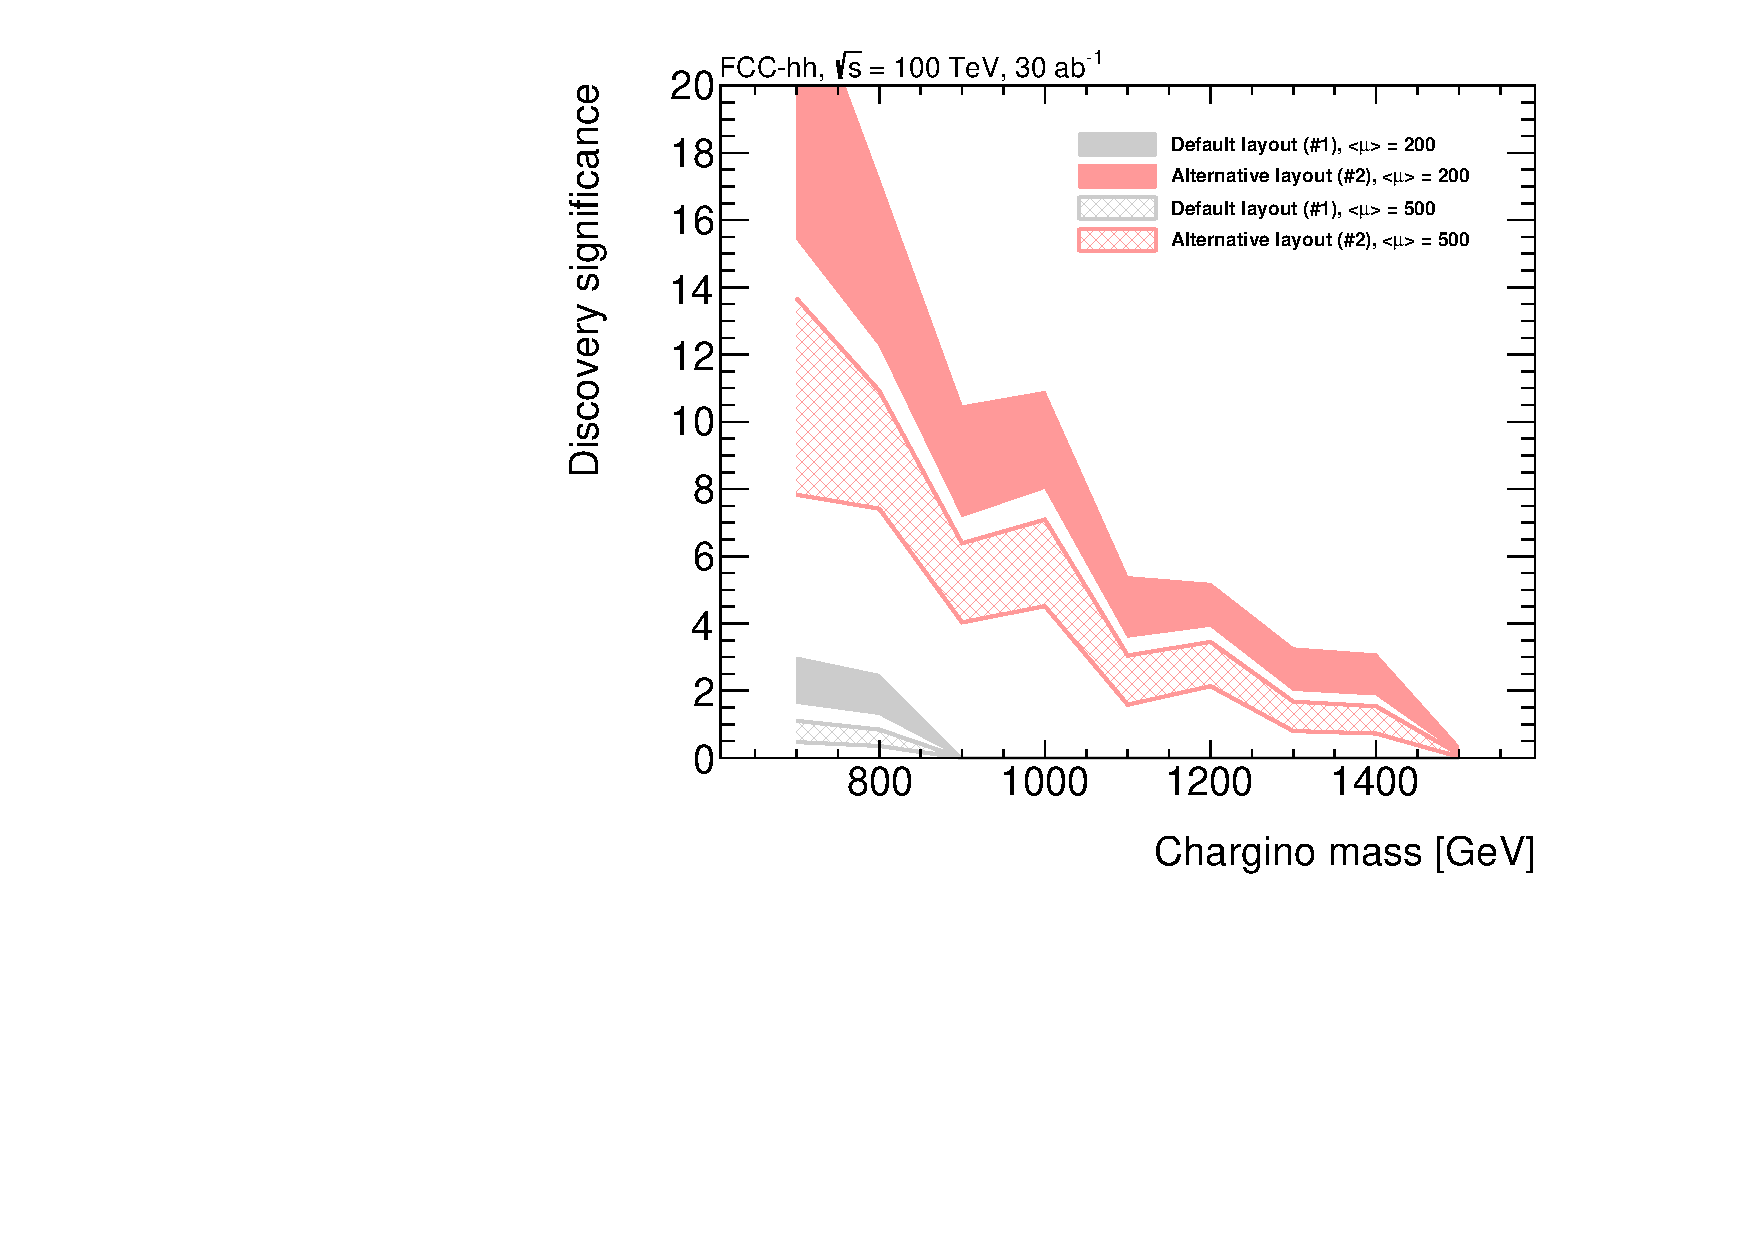
\includegraphics[width=7cm]{\main/experiments/img/h_Significance_di_higgsino9_eta.pdf}
  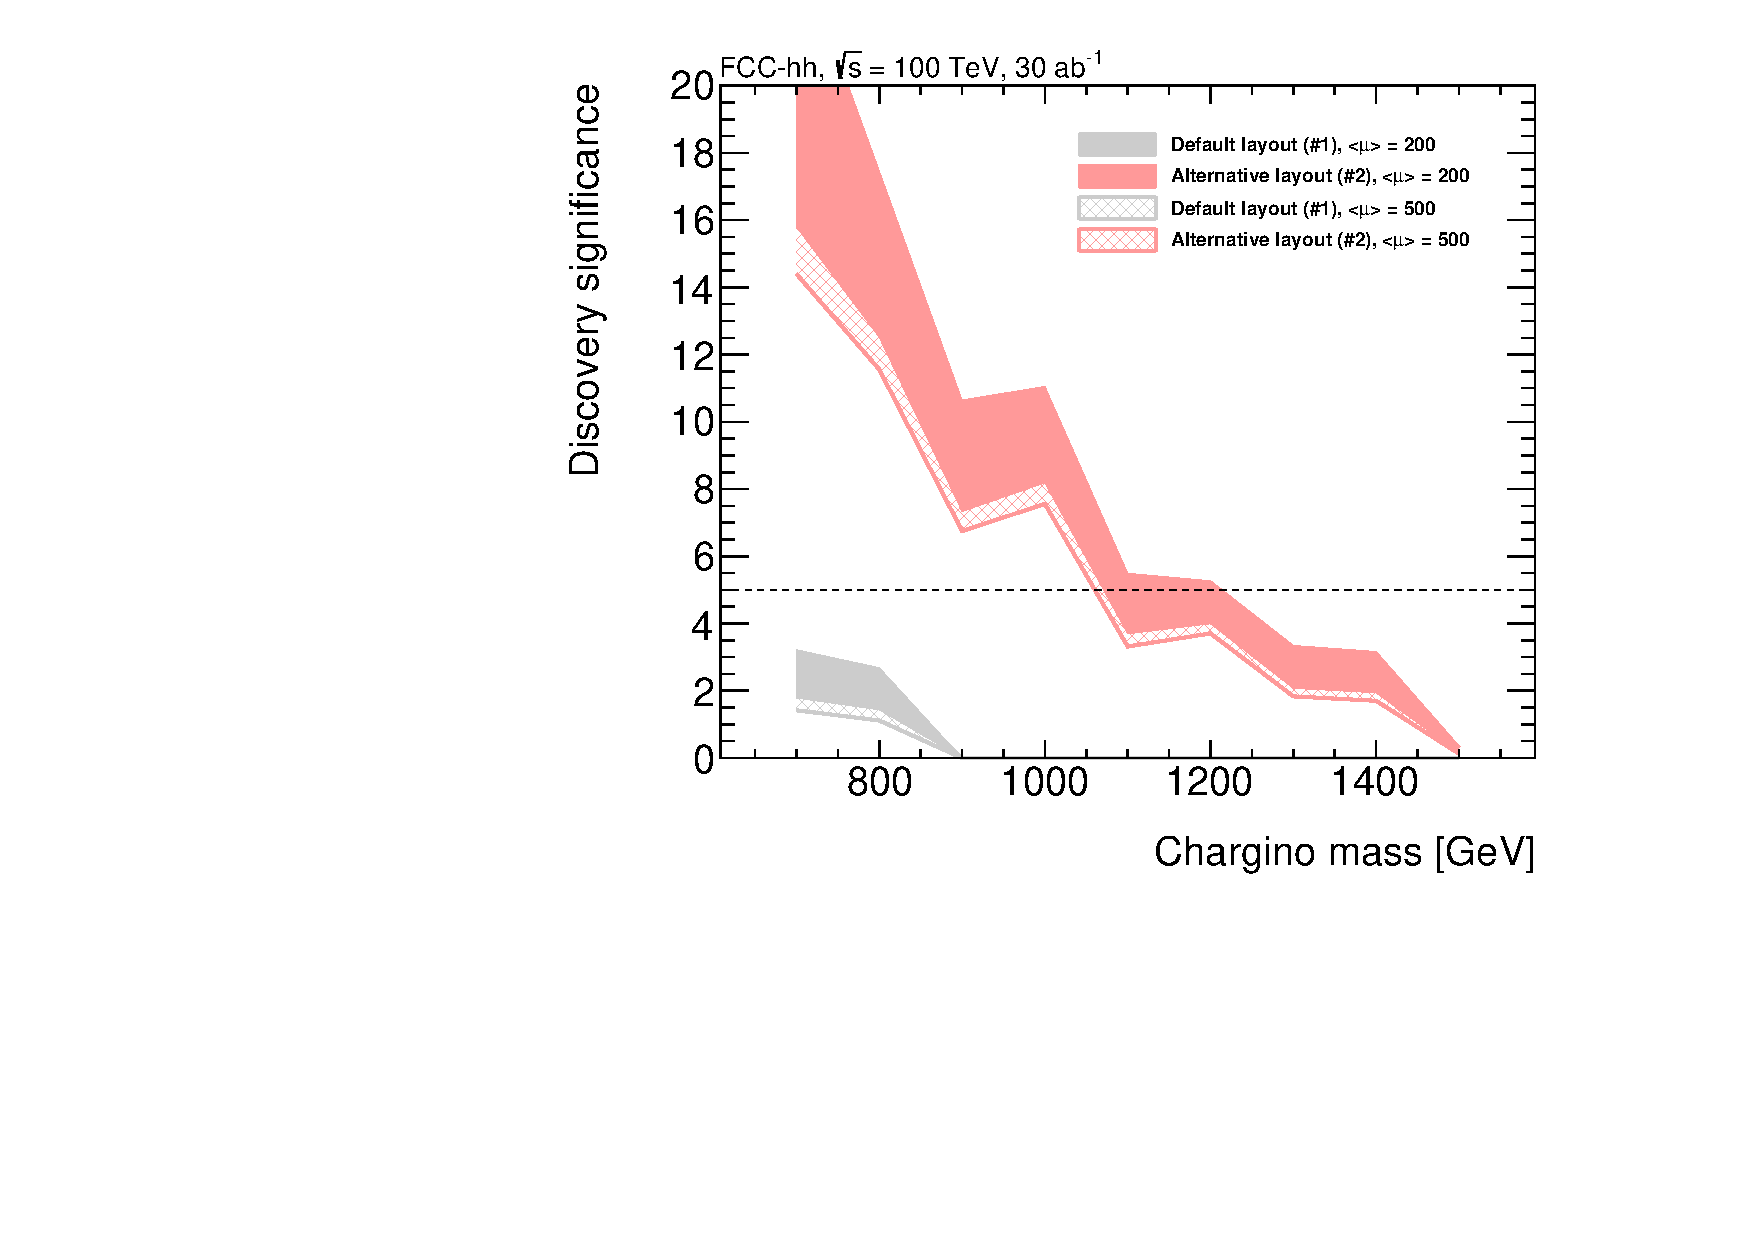
\includegraphics[width=7cm]{h_Significance_higgsino12_eta_5hits.pdf}
  \caption{ a) Wino, $\left< \mu\right>$ {=} 500. b) Higgsino, $\left< \mu\right>$ {=} 200. Expected discovery significance at 30\,ab${}^{-1}$ with requirements of \ensuremath{N_{\mathrm{layer}}^{\mathrm{hit}}}~$\geq$ 5 with 200 (solid) or 500 (hatched) pile-up collisions and $|\eta|<$ 1 with the default (grey) and alternative (red) layouts.
            The band width corresponds to the difference of the two configurations of the soft QCD processes. \MS{need some editing: wino/higgsino have to appear on the plot, thicker 5sigma line, smoothen curve, instead of alternative/default layout write 4-5 pixels tracker...}
          }
  \label{figure:SignificanceEta1}
\end{figure}


\end{document}
